\documentclass[11pt,a4paper]{article}

\usepackage[margin=2.2cm]{geometry}
\usepackage[T1]{fontenc}
\usepackage{lmodern}
\usepackage{graphicx}
\usepackage{booktabs}
\usepackage{amsmath}
\usepackage{xcolor}
\usepackage[font=small,labelfont=bf]{caption}
\usepackage[colorlinks=true,linkcolor=blue!50!black,urlcolor=blue!50!black]{hyperref}

\newcommand{\code}[1]{\texttt{#1}}
\newcommand{\todo}[1]{\textcolor{orange!80!black}{\textbf{[in progress]} #1}}

\title{SPARTA on GPUs for internal-flow DSMC\\\large Working notes on performance}
\author{Nicola Noventa}
\date{\today}

\begin{document}
\maketitle

\begin{abstract}
These notes collect what has been measured so far on the performance of
SPARTA's Kokkos port for the rectangular duct with reservoir case, on single
V100 GPUs and on multi-node CPU runs. The GPU loop is dominated by a single
kernel, the particle move, which runs at low occupancy because it needs about
250 registers per thread. Reordering particles in memory and capping registers
do not help. On CPUs, balancing the grid by particles instead of cells makes the
same run 1.4--1.7$\times$ faster on 1--4 nodes, with a one-line change to the
input deck. The CPU--GPU strong-scaling comparison is in progress.
\end{abstract}

\tableofcontents

%==============================================================================
\section{Setup}
%==============================================================================

\paragraph{Code.} SPARTA with the KOKKOS package, from the fork
\url{https://github.com/NicoNovi9/sparta}. GPU binary: Kokkos CUDA backend,
\code{Kokkos\_ARCH\_VOLTA70}. CPU binary: Kokkos Serial backend, MPI only,
\code{Kokkos\_ARCH\_ZEN4}. Both are built from the same checkout by the scripts
in \code{nicola/compile/}, which record the commit they were built from.
GCC 13.1, HPC-X 2.17.1, CUDA 12.8.

\paragraph{Hardware.}
\begin{itemize}
  \item GPU nodes: 4$\times$ NVIDIA V100 SXM2 32\,GB per node, Skylake host,
        PCIe Gen3 to the host.
  \item CPU nodes (genoaX): AMD EPYC 9684X, 192 cores per node, run with one MPI
        rank per core.
\end{itemize}

\paragraph{Case.} Rectangular duct with reservoir, H$_2$, VSS collisions with
near-neighbour partner selection (\code{collide\_modify nearcp}), subsonic
\code{emit/surf} inlet (10\,Pa) and outlet (5\,Pa), diffuse and specular walls.
Grid $120\times120\times60 = 864{,}000$ cells, of which 269,352 are in the flow,
43,848 are cut by the surface and 550,800 lie outside the flow region;
80,998 surface triangles. Time step $3\times10^{-9}$\,s, \code{stats 100}.
Unless stated otherwise the run starts with 120M particles.

The particle count is not stationary: it drops from 120M to about 97M in the
first 1000 steps, and the collision count drops with it. Timings are therefore
compared over identical step ranges, never as a steady-state rate.

\paragraph{Metric.} \emph{Loop time} is the time SPARTA reports for the time
loop (\code{Loop time of ...}); it excludes setup (grid creation, surface
reading, \code{create\_particles}). Section percentages are SPARTA's own timing
breakdown. GPU kernel times come from Nsight Systems.

%==============================================================================
\section{Profile on a single V100}
%==============================================================================

200 steps, 120M particles, one V100, profiled with Nsight Systems.
Table~\ref{tab:gpu-sections} gives SPARTA's breakdown and
Table~\ref{tab:gpu-kernels} the GPU kernels.

\begin{table}[h]
\centering
\begin{tabular}{lrr}
\toprule
Section & Time [s] & Share \\
\midrule
Move    & 43.52 & 74.8\% \\
Coll    &  5.12 &  8.8\% \\
Output  &  4.76 &  8.2\% \\
Sort    &  4.19 &  7.2\% \\
Modify  &  0.53 &  0.9\% \\
Comm    &  0.08 &  0.1\% \\
\midrule
Loop    & 58.22 & \\
\bottomrule
\end{tabular}
\caption{SPARTA timing breakdown, 120M particles, 200 steps, one V100.}
\label{tab:gpu-sections}
\end{table}

\begin{table}[h]
\centering
\begin{tabular}{lrrr}
\toprule
Kernel & GPU time & Launches & Per launch \\
\midrule
\code{UpdateKokkos::TagUpdateMove}              & 81.2\% & 200 & 216.6\,ms \\
\code{CollideVSSKokkos::TagCollideCollisionsOne}&  8.9\% & 200 &  23.8\,ms \\
\code{ParticleKokkos::TagParticleSort}          &  7.9\% & 203 &  20.8\,ms \\
\code{FixEmitSurfKokkos} (all kernels)          & $<$1\% & 400 &  \\
\bottomrule
\end{tabular}
\caption{GPU kernels by total GPU time (Nsight Systems, same run).}
\label{tab:gpu-kernels}
\end{table}

\begin{itemize}
  \item \textbf{The time loop is GPU-bound.} The kernels add up to 53.3\,s of
        the 58.2\,s loop (about 92\%). The GPU is not waiting for transfers
        during the loop.
  \item \textbf{One kernel dominates.} The particle move is 81\% of GPU time
        and matches SPARTA's \emph{Move} section almost exactly.
  \item \textbf{Output costs a full device-to-host copy.} Every stats output
        synchronises the whole particle array to the host, about 1.5\,s at
        120M particles. In earlier runs (30M particles, 10k steps) this was
        0.55\,s per sync, consistent with PCIe bandwidth, and with
        \code{stats 10} it took 41\% of the loop; reducing the stats frequency
        made the run 1.67$\times$ faster. Upstream pull request \#623 targets
        this sync.
  \item \textbf{Setup is slow.} \code{create\_particles} takes about 100\,s,
        longer than the 200-step loop. The largest host--device copies move the
        whole particle array (12.42\,GB, about 108 bytes per particle) at
        2.6\,GB/s, well below what PCIe Gen3 allows; only two pinned-memory
        allocations appear in the trace, so these copies come from pageable
        memory.
\end{itemize}

%==============================================================================
\section{The move kernel}
%==============================================================================

\subsection{Surface checks are not the problem}
Each particle tests only the triangles of the cell it is in. On average this is
0.749 triangle tests per particle and step over 1.118 cells visited, i.e.\ 0.67
triangles per cell visit. The ratio of tests to actual surface collisions
(about 250:1) only reflects that a wall hit is rare; the culling itself is
already local.

\subsection{Particle order in memory does not matter}
SPARTA never reorders the particle array by cell unless
\code{global particle/reorder} is set. With reordering every 100 steps
(30M particles, 200 steps) the move kernel went from 55.41 to 54.50\,ms per
launch, within noise. Even the fastest launch, with particles freshly created
in cell order, takes 52\,ms, about 7$\times$ the time a purely
bandwidth-limited kernel would need to read and write every particle once.
The kernel is not limited by memory bandwidth or access order.

\subsection{Registers and occupancy}
The instantiation used by this case, \code{TagUpdateMove<3,1,0,0,1>} (3D, with
surfaces), compiles to 252 registers per thread with 288 bytes of stack
(\code{cuobjdump -res-usage}). A V100 SM has 65,536 registers, so only 8 warps
can be resident out of 64: 12.5\% theoretical occupancy, too few warps to hide
memory latency. The variants without surfaces use about 146 registers: the
surface handling compiled into the same kernel roughly doubles the register
count.

Capping the kernel at 128 registers with \code{Kokkos::LaunchBounds} made it
20\% slower (Table~\ref{tab:move}): the stack grew from 288 to 784 bytes per
thread, i.e.\ the compiler spilled to local memory. A build of the fork
without the cap reproduces the previous binary, so the difference is due to
the cap alone.

\begin{table}[h]
\centering
\begin{tabular}{lrrr}
\toprule
Variant (30M particles, 200 steps) & Registers & Stack [B] & Move per launch \\
\midrule
previous binary                     & 252 & 288 & 55.41\,ms \\
particle reorder every 100 steps    & 252 & 288 & 54.50\,ms \\
fork build, unchanged               & 252 & 288 & 55.48\,ms \\
fork build, capped at 128 registers & 128 & 784 & 66.83\,ms \\
\bottomrule
\end{tabular}
\caption{Move kernel experiments on one V100.}
\label{tab:move}
\end{table}

\paragraph{Conclusion.} The move kernel is latency-bound at low occupancy, and
the occupancy is set by the state the kernel carries, not by a compiler
setting. Where it stalls needs Nsight Compute, which is currently blocked
(Section~\ref{sec:open}). A likely direction is to move the surface handling
out of the move kernel, to reduce the register footprint of the common path.

%==============================================================================
\section{Load balancing on CPUs}
%==============================================================================

With $P$ MPI ranks, the grid is split into $P$ pieces, and each rank handles the
particles of its piece. Every step ends only when the slowest rank is done;
the time the others spend waiting appears as \emph{MPI Sync}.

The deck balances with \code{balance\_grid rcb cell}, i.e.\ equal numbers of
cells per rank, and does so before any particle exists. Since 64\% of the
cells lie outside the flow, many ranks get pieces with few or no particles: at
8 nodes some ranks own none at all, while the busiest holds 2.8 times the
average. Adding
\begin{center}
\code{balance\_grid rcb part}
\end{center}
right after \code{create\_particles} rebalances by particle count.
Figure~\ref{fig:balance} and Table~\ref{tab:balance} show the effect.

\begin{figure}[h]
\centering
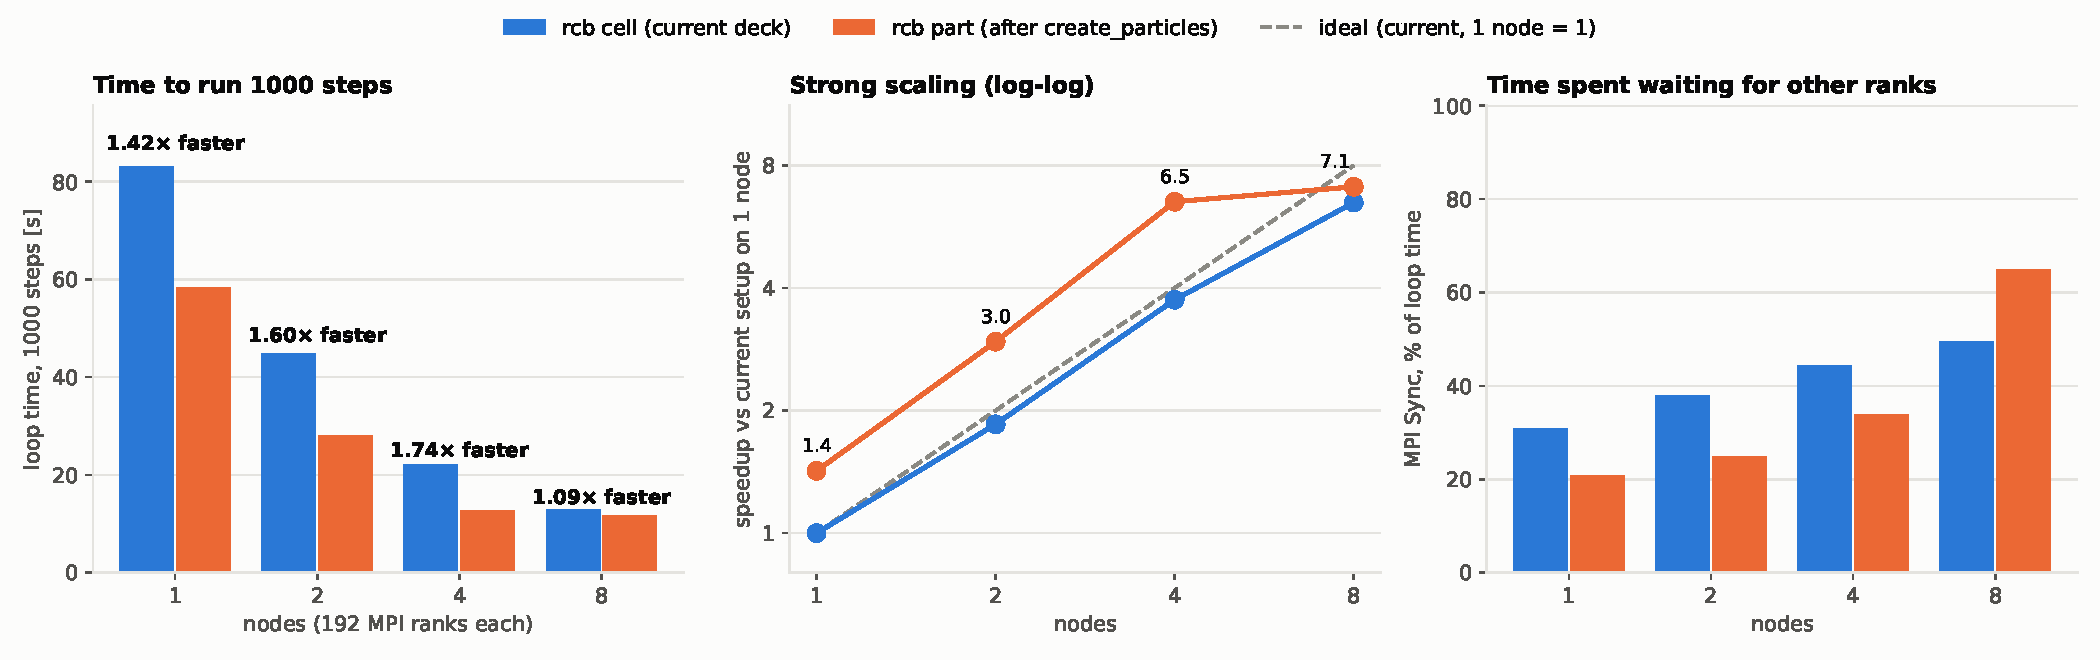
\includegraphics[width=\textwidth]{figures/balance_cpu.pdf}
\caption{Balancing by cells (current deck) versus by particles, genoaX nodes,
192 ranks per node, 120M particles at start, 1000 steps, one run per point.
Left: loop time. Centre: speedup relative to the current setup on one node.
Right: share of the loop spent waiting for other ranks.}
\label{fig:balance}
\end{figure}

\begin{table}[h]
\centering
\begin{tabular}{rrrrrr}
\toprule
Nodes & Ranks & Loop, \code{rcb cell} & Loop, \code{rcb part} & Gain & MPI Sync (cell $\to$ part) \\
\midrule
1 &  192 & 83.05\,s & 58.40\,s & 1.42$\times$ & 30.8\% $\to$ 20.7\% \\
2 &  384 & 44.89\,s & 28.13\,s & 1.60$\times$ & 37.9\% $\to$ 24.8\% \\
4 &  768 & 22.20\,s & 12.76\,s & 1.74$\times$ & 44.4\% $\to$ 33.8\% \\
8 & 1536 & 12.82\,s & 11.73\,s & 1.09$\times$ & 49.4\% $\to$ 64.9\% \\
\bottomrule
\end{tabular}
\caption{Loop time for 1000 steps with the two balancing strategies.}
\label{tab:balance}
\end{table}

\begin{itemize}
  \item On 1--4 nodes the same run is 1.4--1.7$\times$ faster with a one-line
        change to the deck.
  \item With balancing by particles, scaling is superlinear up to 4 nodes
        (4.58$\times$ on 4 nodes relative to 1). A likely reason is that the
        per-node share of the particle data (about 13\,GB in total) increasingly
        fits in the large L3 cache of these CPUs; this has not been measured.
  \item At 8 nodes the gain nearly vanishes. Each step takes about 12\,ms, and
        even the least-waiting rank spends 5.8\,s of the 11.7\,s loop in MPI
        Sync: with about 63k particles per rank, synchronisation dominates
        regardless of balance. This is the strong-scaling limit of this problem
        on CPUs.
  \item The balance is computed once. Whether the gain survives as the gas
        redistributes is being checked with 10,000-step runs.
        \todo{10k-step runs queued.}
\end{itemize}

%==============================================================================
\section{Strong scaling: CPU versus GPU}
%==============================================================================

\todo{GPU runs (1, 2, 4 nodes of 4$\times$V100) are queued.}

Plan: the same deck on 1, 2, 4 (and 8) nodes of each type, 1000 steps; speedup
per architecture, time-to-solution ratio GPU/CPU, and the section breakdown.
Since the GPU runs also balance by cells, they are repeated with
\code{balance\_grid rcb part}, so that balanced CPU runs are compared with
balanced GPU runs.

A first rough comparison: the first 100 steps take 0.10\,s per step on one CPU
node and 0.29\,s per step on a single V100, so one genoaX node is worth about
three V100s on this case.

%==============================================================================
\section{Open issues}
\label{sec:open}
%==============================================================================

\begin{itemize}
  \item \textbf{Nsight Compute is blocked} with \code{ERR\_NVGPUCTRPERM}: GPU
        performance counters are restricted to administrators. Needed to see
        where the move kernel stalls. Request with IT.
  \item \textbf{H200 allocation failure.} On the H200 nodes the run aborts
        after 10--20 steps with a Kokkos \code{BadAlloc} while
        allocating 566.9\,MiB (\code{collide:nn\_last\_partner}) on a 140\,GiB
        GPU holding 6.4\,GB; the same job completes on a V100. Ticket open
        with IT.
  \item \textbf{GPU-aware MPI} is assumed by SPARTA without checking; to be
        confirmed by the first multi-GPU runs.
  \item \textbf{Particles per cell.} 120M particles in 313,200 flow cells is
        about 380 particles per cell at start, far above the $\geq 20$ usually
        required. If the physics allows fewer, the cost drops proportionally.
  \item \textbf{Deck order.} \code{global gridcut} is set after
        \code{create\_grid}, so every rank keeps the whole grid (138\,MB per
        rank). Harmless at the current sizes.
  \item \textbf{Pinned memory} for the host--device copies could make setup
        and output syncs up to about 4$\times$ faster.
\end{itemize}

\end{document}
